\documentclass[
    % handout,
    center,
    % aspectratio=169
]{beamer}

\usepackage[utf8]{inputenc}
\usepackage[english]{babel}
\usepackage{graphicx}
\usepackage{booktabs}
\usepackage{tabularx}
\usepackage[ruled,vlined]{algorithm2e}

\graphicspath{../}

\title[Deep Learning Camera Pose Estimation]{\textsc{A Deep Learning Approach to\\Camera Pose Estimation}}
\author[Bozzo - Izzo]{Federico Izzo \and Francesco Bozzo}
\institute[UniTN]{University of Trento}
\date{January 12, 2022}

% \logo{\includegraphics[height=1.5cm]{logo.png}}
\usetheme{Madrid}
\definecolor{links}{HTML}{54489a}
\hypersetup{colorlinks,linkcolor=,urlcolor=links}
% \usetheme{metropolis} 


\begin{document}

\begin{frame}
    \titlepage
\end{frame}

% \AtBeginSection[]
% {
%     \begin{frame}{Table of Contents}
%         \begin{columns}[t]
%             \column{.45\textwidth}
%             \tableofcontents[sections=1-2, currentsection]

%             \column{.45\textwidth}
%             \tableofcontents[sections=3-5, currentsection]
%         \end{columns}
%     \end{frame}
% }

\section{Introduction}
\begin{frame}{Introduction}
    With this work we are going to present:
    \begin{itemize}
        \item the exploration of multiple dataset generation techniques;
        \item the COLMAP reconstruction of Povo 1 second floor;
        \item the development of relative and absolute pose estimation models;
        \item the fine-tuning of absolute pose estimation models;
        \item the post-processing of the model outputs;
        \item the model deployment using a FastAPI web-server. 
    \end{itemize}
\end{frame}

\section{Dataset}

\section{Models}
\subsection{MeNet}
\begin{frame}{The MeNet Model for Relative Pose Estimation}
    \begin{columns}
        \column{0.45\textwidth}
        \begin{figure}
            \centering
            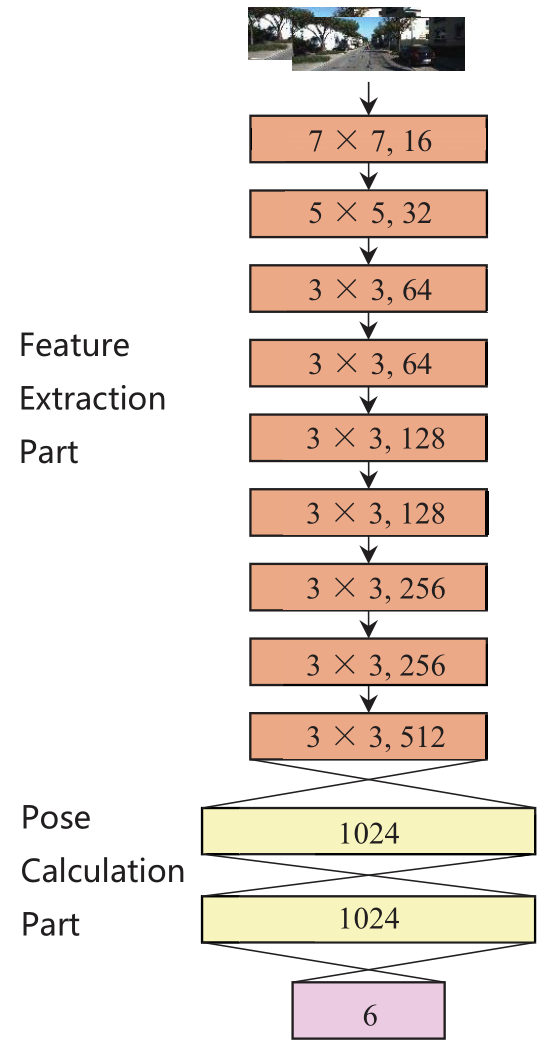
\includegraphics[width=0.9\textwidth]{../imgs/menet_structure.png}
            \caption{MeNet model architecture.}
        \end{figure}

        \column{0.45\textwidth}
        The \textbf{MeNet} model is targeted for \textbf{relative pose estimation}.
        The input of the network consists in a stack of two images: the goal is to estimate the relative pose of the second image with respect to the first one.
    \end{columns}
\end{frame}
\subsection{PoseNet}
\begin{frame}{The PoseNet Model for Absolute Pose Estimation}
    \begin{columns}
        \column{0.45\textwidth}
        \begin{figure}
            \centering
            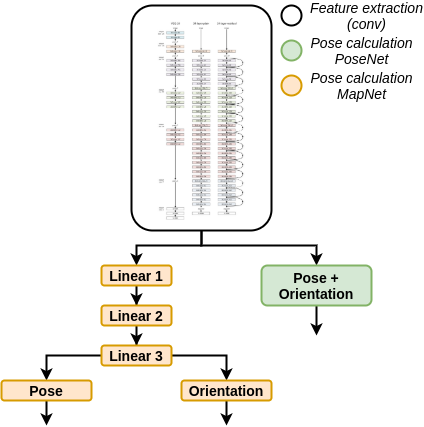
\includegraphics[width=0.9\textwidth]{../imgs/mapnet_posenet_structure.png}
            \caption{PoseNet model architecture.}
        \end{figure}

        \column{0.45\textwidth}
        The \textbf{PoseNet} model for absolute pose estimation is made up by two components:
        \begin{itemize}
            \item feature extraction through a sequence of convolutional layers (\emph{backend});
            \item pose regression on the extracted features using linear layers.
        \end{itemize}
    \end{columns}
\end{frame}

\subsection{MapNet}
\begin{frame}{The MapNet Model for Absolute Pose Estimation}
    \begin{columns}
        \column{0.45\textwidth}
        \begin{figure}
            \centering
            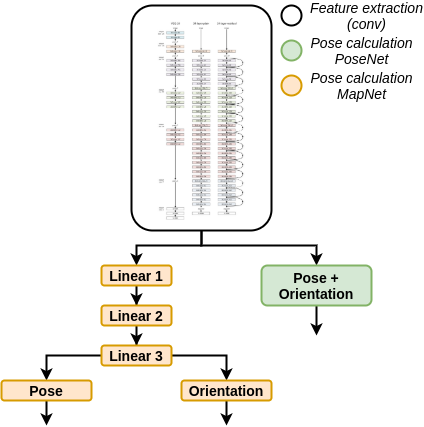
\includegraphics[width=0.9\textwidth]{../imgs/mapnet_posenet_structure.png}
            \caption{MapNet model architecture.}
        \end{figure}

        \column{0.45\textwidth}
        The \textbf{MapNet} model for absolute pose estimation represents an evolution of the PoseNet model with improvements:
        \begin{itemize}
            \item increase the number of final linear layers;
            \item penalize both absolute and relative errors in the loss.
        \end{itemize}
    \end{columns}
\end{frame}

\section{Conclusions}
\begin{frame}{Conclusions}
    To summarize, the final results presented in this work are:
    \begin{itemize}
        \item the exploration of multiple dataset generation techniques;
        \item the COLMAP reconstruction of Povo 1 second floor;
        \item the development of relative and absolute pose estimation models;
        \item the fine-tuning of absolute pose estimation models;
        \item the post-processing of the model outputs;
        \item the model deployment using a FastAPI web-server. 
    \end{itemize}
\end{frame}

% \begin{frame}{Block examples}
%     \begin{block}{Observation 1}
%         Simmons Hall is composed of metal and concrete.
%     \end{block}
%     \begin{exampleblock}{Observation 2}
%         Simmons Hall is composed of metal and concrete.
%     \end{exampleblock}
%     \begin{textbfblock}{Conclusion}
%         Simmons Hall $\not=$ Simmons Dormitory.
%     \end{textbfblock}
% \end{frame}
\end{document}
